% kuleuventheme2 by Janez Kren, September 2017, janez.kren@kuleuven.be, based on:
% kuleuventheme 1.3 by Roland Pastorino, 2013 roland.pastorino@kuleuven.be / www.rolandpastorino.com

\documentclass[11pt,t]{beamer}
\usetheme{kuleuven2}	%THEME OPTIONS for LOGO: kul (default), kulak, lrd,    ; OPTIONS for TITLE PAGE: normal (default), sedes
\useoutertheme{miniframes}  % Adds the circle slide indicators at the top
\let\AtBeginSection\relax    % Disable automatic outline slides

%%% OTHER SETTINGS
\usefonttheme[onlymath]{serif}			% math font with serifs, delete to make it sans-serif
\setbeamertemplate{footline}[body] 		% delete this line to remove footline bar on all frames
%\usepackage[orientation=landscape,size=custom,width=16,height=9,scale=0.5,debug]{beamerposter} %enable for widescreen 16:9 ratio


%%% ADDED PACKAGES:
\usepackage[english]{babel}
\usepackage{amsfonts}
\usepackage{amssymb}


%%% TITLE PAGE INFO:
\title[`AIMD' Simulations of Phosphate Hydrolysis Using NNPs]{\textit{Ab Initio} Molecular Dynamics Simulations of Phosphate Hydrolysis Using Neural Network Potentials} %[]] will appear in footline
\subtitle{Master's thesis defence presentation}
\setlength{\fboxrule}{0.3pt}
\setlength{\fboxsep}{0pt}
\titlegraphic{%
  \raisebox{-4.1cm}{\fbox{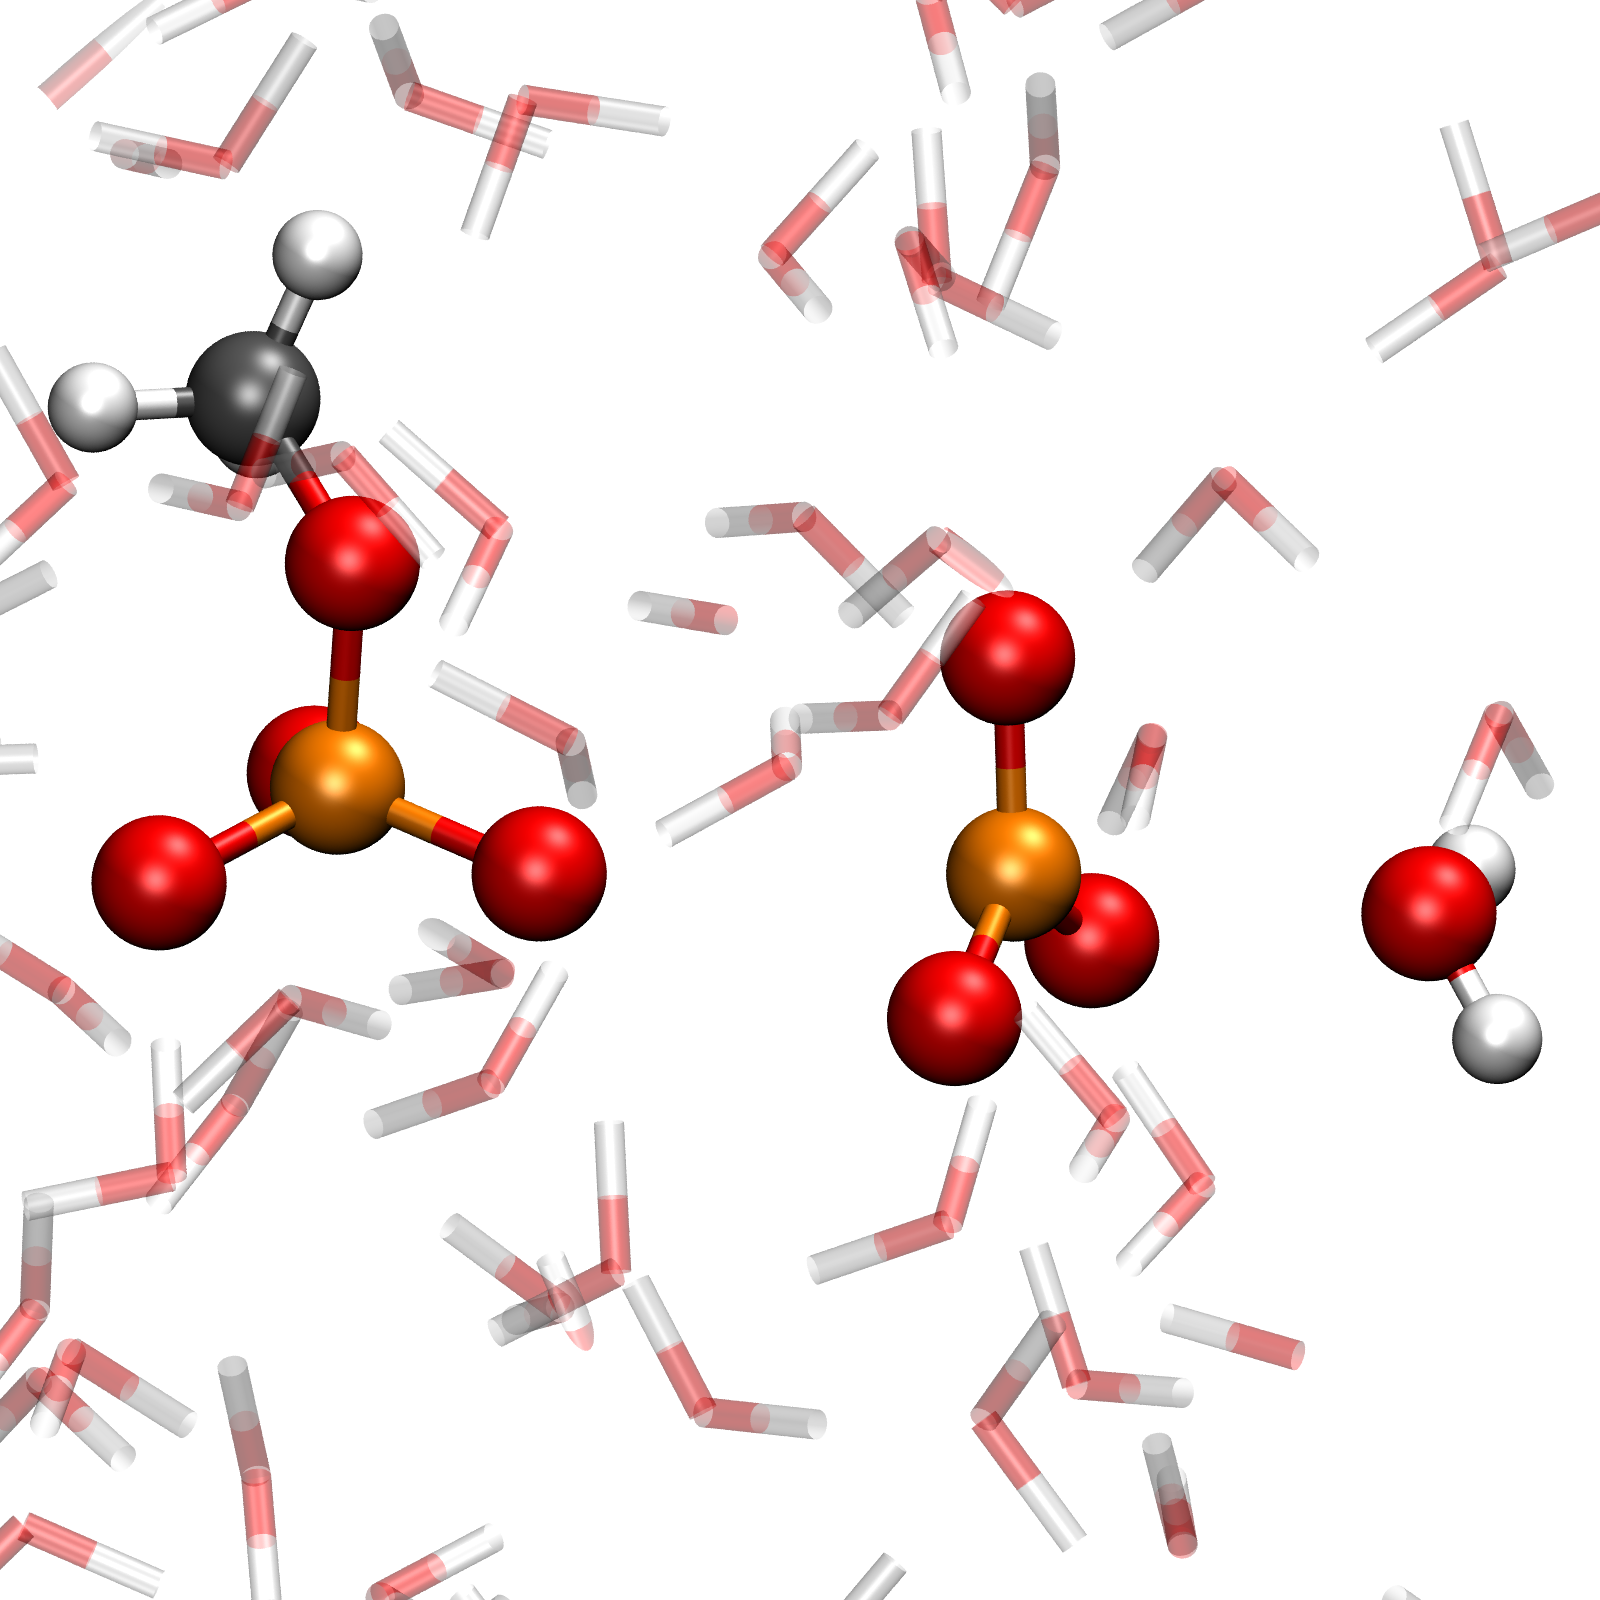
\includegraphics[width=.18\paperwidth]{Figures/MeDP_TSdissoc.png}}}
}
\author{Albert Makhmudov}
\institute{Supervisor: Prof. J. Harvey}
\date{June 2025}



\begin{document}
\csname beamer@calculateheadfoot\endcsname %recalculate head and foot dimension



 %%
 %%  0. TITLE PAGE and TABLE OF CONTENT
 %%
% Title page
\begin{frame}[plain,noframenumbering]
	\titlepage
\end{frame}



 %%
 %%  SECTION 1 - INTRODUCTION
 %%
\section{Introduction}
\begin{frame}{Why is phosphate hydrolysis challenging to study?}
	\vspace{-30pt}
	\begin{figure}
		\centering
		\includegraphics[width=0.9\textwidth]{Figures/introduction_background.png}
		\small
		\flushleft
		Would be nice to include a take-home message.
	\end{figure}
\end{frame}



\begin{frame}{Research goals}
	\small
	\begin{itemize}
		\item Compose a comprehensive dataset covering all reaction steps.
		\item Train the NequIP neural network to fit a neural network potential (NNP).
		\item Assess the accuracy and performance of the NNP.
		\item Perform well-tempered metadynamics simulations to obtain the free energy surface.
		\item Gain insights into the kinetics and thermodynamics of the reaction.
		\item Gain insights into the proton transfer mechanism.
	\end{itemize}	
\end{frame}



\begin{frame}
	\vspace{0.5cm}
	\begin{figure}
		\centering
		\includegraphics[width=0.23\textwidth]{Figures/introduction_paul_dirac.jpg}
	\end{figure}
	\small
	\begin{quotation}
		It therefore becomes desirable that approximate practical methods of applying quantum mechanics should be developed, which can lead to an explanation of the main features of complex atomic systems \textbf{without too much computation}.

		\raggedleft	\normalfont --  Paul Dirac
	\end{quotation}
\end{frame}



 %%
 %%  SECTION 2 - THEORETICAL BACKGROUND
 %%
\section{Theoretical background}
\begin{frame}{Geometric graph neural networks}
	\vspace{-10pt}
	\begin{figure}
		\centering
		\includegraphics[width=0.9\textwidth]{Figures/theory_geometric_gnns.png}
	\end{figure}
	\small
	Would be nice to include a take-home message.
\end{frame}



\begin{frame}{Neural equivariant interatomic potentials (NequIP)}
	\small
	The neural network is trained using a loss function:
	\begin{gather*}
		\mathcal{L} = \lambda_E \lVert \hat{E} - E \rVert^2 + \lambda_F \frac{1}{3N} \sum_{i=1}^{N} \sum_{\alpha=1}^{3} \left\lVert -\frac{\partial \hat{E}}{\partial r_{i,\alpha}} - F_{i,\alpha} \right\rVert^2
		\label{eq:loss_function}
	\end{gather*}
	It is based on a weighted sum of energy and force loss terms. Where $\hat{E}$ is the predicted energy, $\lambda_E$ and $\lambda_F$ are the energy and force weights, respectively, and $N$ is the number of atoms. MSE loss is used.
	\begin{figure}
		\centering
		\includegraphics[width=0.55\textwidth]{Figures/theory_nequip.png}
	\end{figure}
\end{frame}



\begin{frame}{Metadynamics}
	\vspace{-10pt}
	\begin{figure}
		\centering
		\includegraphics[width=0.9\textwidth]{Figures/theory_metadynamics.png}
	\end{figure}
	\small
	Would be nice to include a take-home message.
\end{frame}



 %%
 %%  SECTION 3 - METHODOLOGY
 %%
\section{Methodology}
\begin{frame}{System}
	\vspace{-5pt}
	\begin{figure}
		\centering
		\includegraphics[width=0.9\textwidth]{Figures/methods_collective_variables.png}
	\end{figure}
	\small
	The systems studied in this work are the following:
	\begin{itemize}
		\item MeDP$^{3-}$ with 3 Na$^+$ counterions solvated by 119 H$_2$O.
		\item MeHDP$^{2-}$ with 2 Na$^+$ counterions solvated by 124 H$_2$O.
	\end{itemize}
	The box dimensions are 15.877 $\times$ 15.877 $\times$ 15.877 and 15.901 $\times$ 15.901 $\times$ 15.901 \AA$^3$, respectively.
\end{frame}



\begin{frame}{Neural network training workflow}
	\vspace{-10pt}
	\begin{figure}
		\centering
		\includegraphics[width=1.0\textwidth]{Figures/methods_workflow_diagram.pdf}
	\end{figure}
\end{frame}



 %%
 %%  SECTION 4 - RESULTS
 %%
\section{Results}
\begin{frame}{Final training and test datasets' composition}
	\vspace{-10pt}
	\begin{figure}
		\centering
		\includegraphics[width=0.85\textwidth]{Figures/results_final_dataset_with_histograms.png}
	\end{figure}
	\small
	The final training and test datasets consist of 12,000 and 1,800 frames, respectively, and covers all reaction steps.
\end{frame}



\begin{frame}{Accuracy of the fitted potential}
	\begin{columns}[t]
		\begin{column}{.55\textwidth}
			\vspace{-20pt}
			\begin{figure}
				\centering
				\includegraphics[width=1.0\textwidth]{Figures/results_nnp_accuracy_l-1_l-2.png}
			\end{figure}	
		\end{column}
		\begin{column}{.45\textwidth}
			\small
			Community standards are as follows:
			\begin{itemize}
				\item `very good fit' \\
				\noindent $\text{MAE}_E = 1\text{-}10 \; \text{meV/atom}$ \\
				\noindent $\text{RMSE}_F = 20\text{-}40 \; \text{meV/\AA}$
				\item `perfect fit' \\
				\noindent $\text{MAE}_E \sim 1 \; \text{meV/atom}$ \\
				\noindent $\text{RMSE}_F \sim 10 \; \text{meV/\AA}$
			\end{itemize}
			We fitted 2 potentials and both of them are very accurate exhibiting fairly small errors.
		\end{column}
	\end{columns}	
\end{frame}



\begin{frame}{Performance of the potential}
	\vspace{-10pt}
	\begin{figure}
		\centering
		\includegraphics[width=0.6\textwidth]{Figures/results_performance_comparison.png}
	\end{figure}
	\small
	The $\ell = 1$ potential is about 2.5 times faster than the $\ell = 2$ potential, while the accuracy is comparable.
\end{frame}



\begin{frame}{Convergence of the free energy profiles}
	\begin{columns}[t]
		\begin{column}{.65\textwidth}
			\vspace{-25pt}
			\begin{figure}
				\centering
				\includegraphics[width=1.05\textwidth]{Figures/results_300K_fes_conv_cv_evol.png}
			\end{figure}	
		\end{column}
		\begin{column}{.35\textwidth}
			\vspace{-10pt}
			\small
			\begin{itemize}
				\item The profiles are not fully converged.
				\item Hence, the results should be considered provisional.
				\item There are recrossing events between the reactants and products states.
				\item Which gives confidence in the soon approaching convergence.
			\end{itemize}
		\end{column}
	\end{columns}
\end{frame}



\begin{frame}{Reaction mechanism for MeDP$^{3-}$ at 300 K}
	\vspace{-10pt}
	\begin{figure}
		\centering
		\includegraphics[width=0.9\textwidth]{Figures/results_MeDP_300K_fes_mfep.png}
	\end{figure}
	\small
	$\Delta G^\ddagger_\text{exp}$ for HP$_2$O$_7$$^{3-}$ hydrolysis at 25\textdegree{C} is 29.2 kcal/mol. $\Delta G^\ddagger_\text{calc}$ of 28.22 kcal/mol for the D$_\text{N}$A$_\text{N}$ mechanism is within the chemical accuracy!
\end{frame}



\begin{frame}
	\vspace{-10pt}
	\begin{figure}
		\centering
		\includegraphics[width=0.95\textwidth]{Figures/results_MeDP_reaction_mechanism_steps.pdf}
	\end{figure}
	\small
	Would be nice to include a take-home message.
\end{frame}



\begin{frame}{Proton transfer mechanism}
	\vspace{-10pt}
	\begin{figure}
		\centering
		\includegraphics[width=0.9\textwidth]{Figures/results_proton_transfer.pdf}
	\end{figure}
	\small
	Would be nice to include a take-home message.
\end{frame}



 %%
 %%  SECTION 5 - CONCLUSIONS
 %%
\section{Conclusions}
\begin{frame}{What we achieved so far?}
	\begin{columns}[t]
		\begin{column}{.55\textwidth}
		\vspace{-10pt}
		\small
		\begin{itemize}
			\item The NNP produced expected for the PBE-D3(BJ)/TZV2P results.
			\item For the first time, the 2 ns long sampling was performed.
			\item MeDP$^{3-}$ hydrolysis goes through the D$_\text{N}$A$_\text{N}$ mechanism.
			\item The agreement with the experiment is excellent.
			\item The proton transfer mechanism involving 1 and 3 water molecules was shown.
		\end{itemize}	
		\end{column}
		\begin{column}{.45\textwidth}
			\vspace{-25pt}
			\begin{figure}
				\centering
				\includegraphics[width=1.0\textwidth]{Figures/conclusions_mfj_plot.png}
			\end{figure}
			\centering
			\scriptsize
			More O'Ferral Jencks diagram for MeDP$^{3-}$ hydrolysis.
		\end{column}
	\end{columns}
\end{frame}



 %%
 %%  SECTION 6 - OUTLOOK
 %%
\section{Outlook}
\begin{frame}{What can be done further?}
	\begin{columns}[t]
		\begin{column}{.65\textwidth}
		\vspace{-10pt}
		\small
		\begin{itemize}
			\item Extended sampling to reach the convergence.
			\item Transition state validation.
			\item Effect of enthalpy and entropy.
			\item Extension to more complex systems.
		\end{itemize}
		\textit{As neural network potentials continue to improve, they are likely to become an indispensable tool in the computational chemist's toolkit, enabling the exploration of chemical space with unprecedented accuracy and efficiency.}	
		\end{column}
		\begin{column}{.35\textwidth}
			\vspace{-30pt}
			\begin{figure}
				\centering
				\includegraphics[width=0.9\textwidth]{Figures/outlook_atp_synthase.pdf}
			\end{figure}
		\end{column}
	\end{columns}
\end{frame}



 %%
 %%  SECTION 7 - ACKNOWLEDGMENTS
 %%
\section{Acknowledgments}
\begin{frame}{Thank you for your attention!}
	\footnotesize
	Acknowledgments:
	\begin{itemize}
	\item Jeremy Harvey and all members of the research group, as well as the QCPC division;
	\item Ehsan Moravveji (VSC), Hans Vansweevelt (KUL), and Anders Johansson (Harvard) for technical assistance;
	\item TCCM cohort for the coffee breaks, lunches, and a lot of fun times we shared in 2 years;
	\item EMJMD TCCM for the financial support by means of Erasmus+ scholarship.
	\end{itemize}
	\begin{figure}
		\centering
		\includegraphics[width=0.95\textwidth]{Figures/acknowledgments.pdf}
	\end{figure}
	\small
	Would be nice to include a take-home message.
\end{frame}



\end{document}